\subsection{Reengineered Task Organization Model}
Das Reengineered Task Organization Model repräsentiert die Arbeit der Benutzer mithilfe des zu entwicklende System. Die Abbildung \ref{img:reengineeredTaskOrganizationModel}: \nameref{img:reengineeredTaskOrganizationModel} beschreibt den Prozess der Arbeit des Diabetikers mit dem System anhand der Concrete Use Cases aus der Aufgebenmodellierung und ergänzt das Task Organization Model. Alle Erkenntisse aus der Aufgabenmodellierung fließen zunächst in das Reengineered Task Organization Model und folglich auch in das Design der Screens ein.
\begin{figure}[H]
	\centering
	\setlength{\fboxsep}{1pt}
	\setlength{\fboxrule}{1pt}
	\fbox{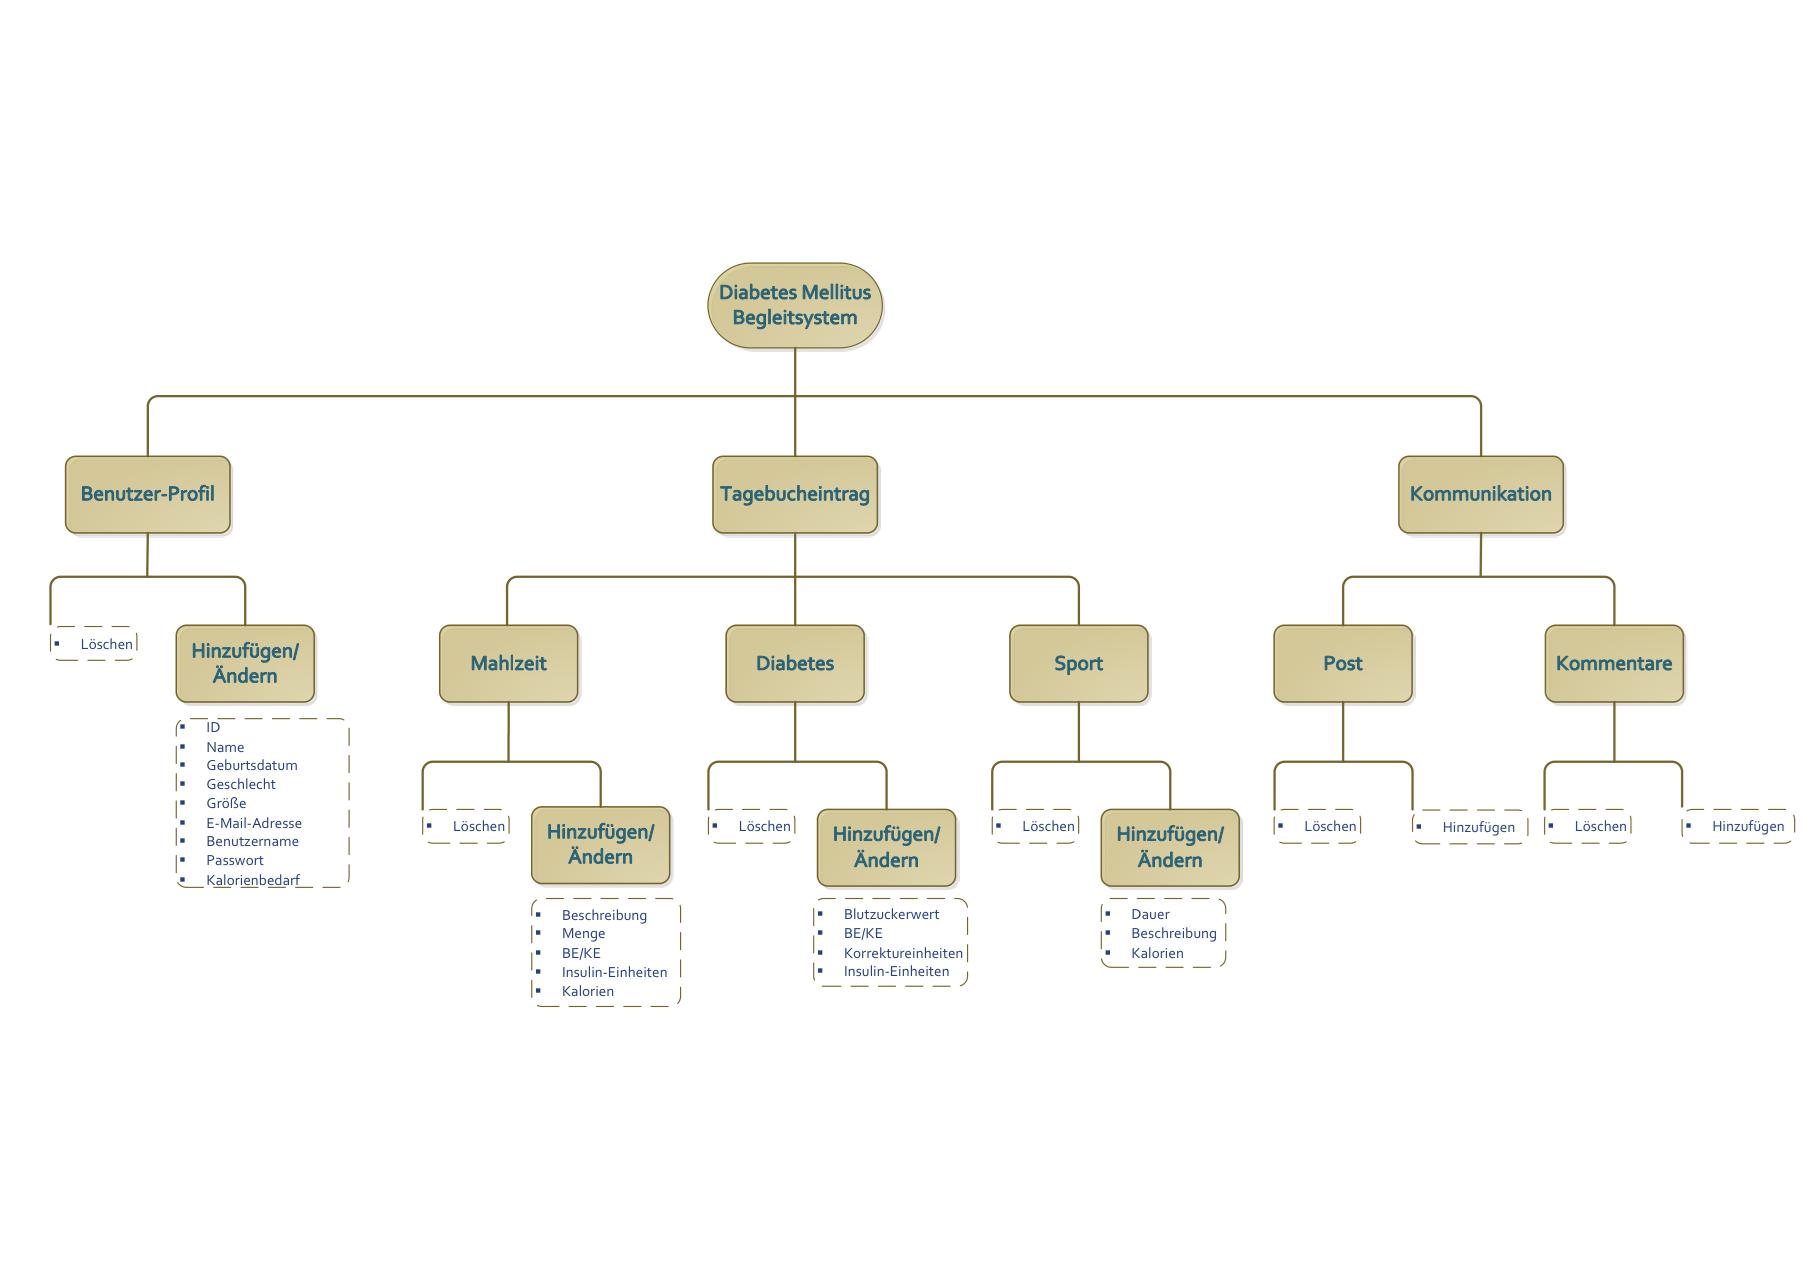
\includegraphics[width=1.0\textwidth]{images/reengineeredTaskOrganizationModel.png}}
	\captionsetup{justification=centering}
	\caption{Reengineered Task Organization Model}
	\label{img:reengineeredTaskOrganizationModel}
\end{figure}
\subsection{Conceptual Model (CM) Design}
Im Concetpual Model Design werden erste Screens für das zu entwickelnde System designt. Die ersten groben Entwürfe sollen den Navigationspfad und die Haupt-Screens identifizieren und anhand dessen erste Regeln für das finale Design des Interfaces festlegen. Ziel ist hier jedoch nicht ein detailreiches Interface Design zu bestimmen. Dieses Design muss zunächst in den kommenden Designaufgaben entwickelt werden.\\
Nach Mayhew \cite{MD} muss zunächst bestimmt werden, ob es sich bei dem Conceputal Model Design um ein product- oder process-oriented model handelt. Da es in dem zu entwickelnde System keine Arbeitsprodukte, welche vom Benutzer individuell erstellt oder bearbeitet werden. In diesem System sollen die Arbeitsprozesse von Diabetikern unterstützt werden. Auf Informationen wie die Nährwerte von Lebensmitteln haben alle Benutzer Zugriff, können abgerufen und in ihrem Tagebuch gespeichert werden. Aufgrund dessen handelt es sich in diesem Fall um ein process-oriented model.\\
In nächsten Schritt sind die Prozesse des process-oriented model zu identifizieren. Bei einem process-oriented model definiert das \nameref{img:reengineeredTaskOrganizationModel} auf Seite \pageref{img:reengineeredTaskOrganizationModel} die (Unter-)Prozesse des Systems und aus diesem lässt sich folgende Aufgabenhierarchie ableiten:\\
Benutzer\newline
\noindent\hspace*{10mm}Benutzer hinzufügen\newline
\noindent\hspace*{10mm}Benutzer bearbeiten\newline
\noindent\hspace*{10mm}Benutzer löschen\newline
Tagebuch\newline
\noindent\hspace*{10mm}Blutzuckerwert\newline
\noindent\hspace*{20mm}Blutzuckerwert hinzufügen\newline
\noindent\hspace*{20mm}Blutzuckerwert bearbeiten\newline
\noindent\hspace*{20mm}Blutzuckerwert löschen\newline
\noindent\hspace*{10mm}Mahlzeit\newline
\noindent\hspace*{20mm}Mahlzeit hinzufügen\newline
\noindent\hspace*{20mm}Mahlzeit bearbeiten\newline 
\noindent\hspace*{20mm}Mahlzeit löschen\newline
\noindent\hspace*{10mm}Aktivität\newline
\noindent\hspace*{20mm}Aktivität hinzufügen\newline
\noindent\hspace*{20mm}Aktivität bearbeiten\newline
\noindent\hspace*{20mm}Aktivität löschen\newline
Kommunikation\newline
\noindent\hspace*{10mm}Beitrag\newline
\noindent\hspace*{20mm}Beitrag hinzufügen\newline
\noindent\hspace*{20mm}Beitrag löschen\newline
\noindent\hspace*{10mm}Kommentar\newline
\noindent\hspace*{20mm}Kommentar hinzufügen\newline
\noindent\hspace*{20mm}Komentar löschen\\
Um nun die Darstellungregeln für die Prozesse zu gestalten wird eine Bottom-Navigation-Bar verwendet. Die Navigation könnte wie in Abbildung \ref{img:navigationbar}: \nameref{img:navigationbar} dargestellt werden. \newline
Für eine Bottom-Navigation-Bar wurde sich entschieden, um den Benutzer Kontrolle über das System und eine gewisse Freiheit zu gewährleisten. So ermöglicht das System dem Benutzer bei versehentlicher Auswahl einer Navigation einen deutlich gekennzeichneten „Notausgang“, indem der Benutzer lediglich durch die Bottom-Navigation den unerwünschten Systemzustand verlässt, ohne einen erweiterten Dialog durchlaufen zu müssen.
\begin{figure}[H]
	\centering
	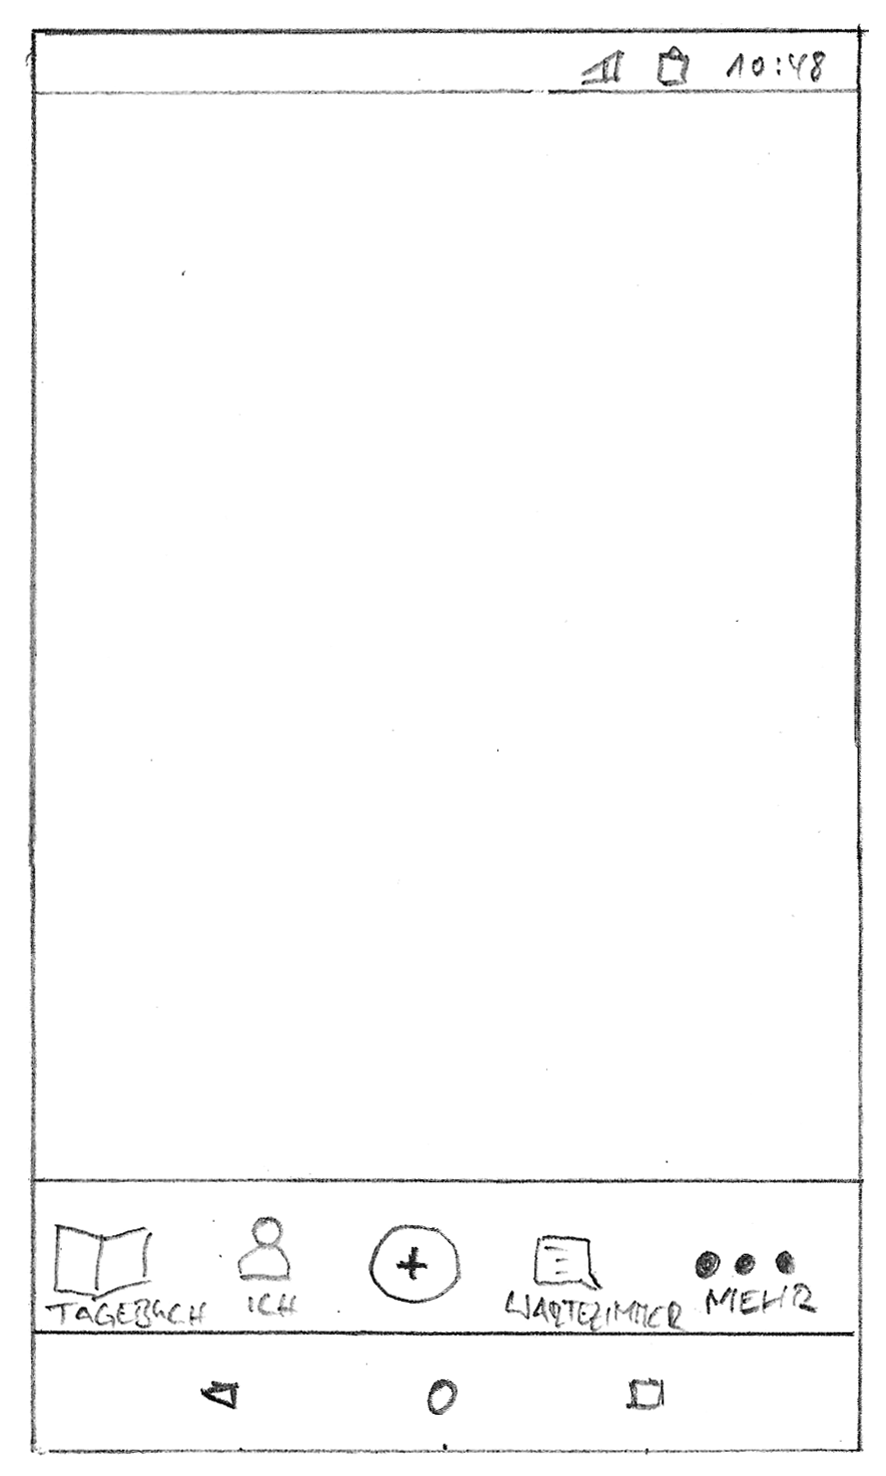
\includegraphics[width=0.3\textwidth]{images/navigationbar.png}
	\captionsetup{justification=centering}
	\caption{Bottom-Navigation-Bar}
	\label{img:navigationbar}
\end{figure}
Unter dem Navigationspfad „Tagebuch“ (Abbildung \ref{img:tagebuchscreen}: \nameref{img:tagebuchscreen})sind Blutzuckerwerte, Mahlzeiten und Aktivitäten anzulegen, zu bearbeiten, einzusehen und zu löschen. Unter „Ich“ (Abbildung \ref{img:ichscreen}: \nameref{img:ichscreen}) und „Mehr“ (Abbildung \ref{img:mehrscreen}: \nameref{img:mehrscreen}) können Benutzerkonten eingesehen, bearbeitet und gelöscht werden und im „Wartezimmer“ (Abbildung \ref{img:wartezimmerscreen}: \nameref{img:wartezimmerscreen}) sind Beiträge und Kommentage einzusehen, hinzuzufügen und zu löschen. Das Plus-Icon ermöglich zusätzlich das hinzufügen von Blutzuckerwerten, Mahlzeiten, Aktivitäten und Beiträge. So könnten die Screens folgendermaßen dargestellt werden. 
\begin{figure}[H]
	\centering
	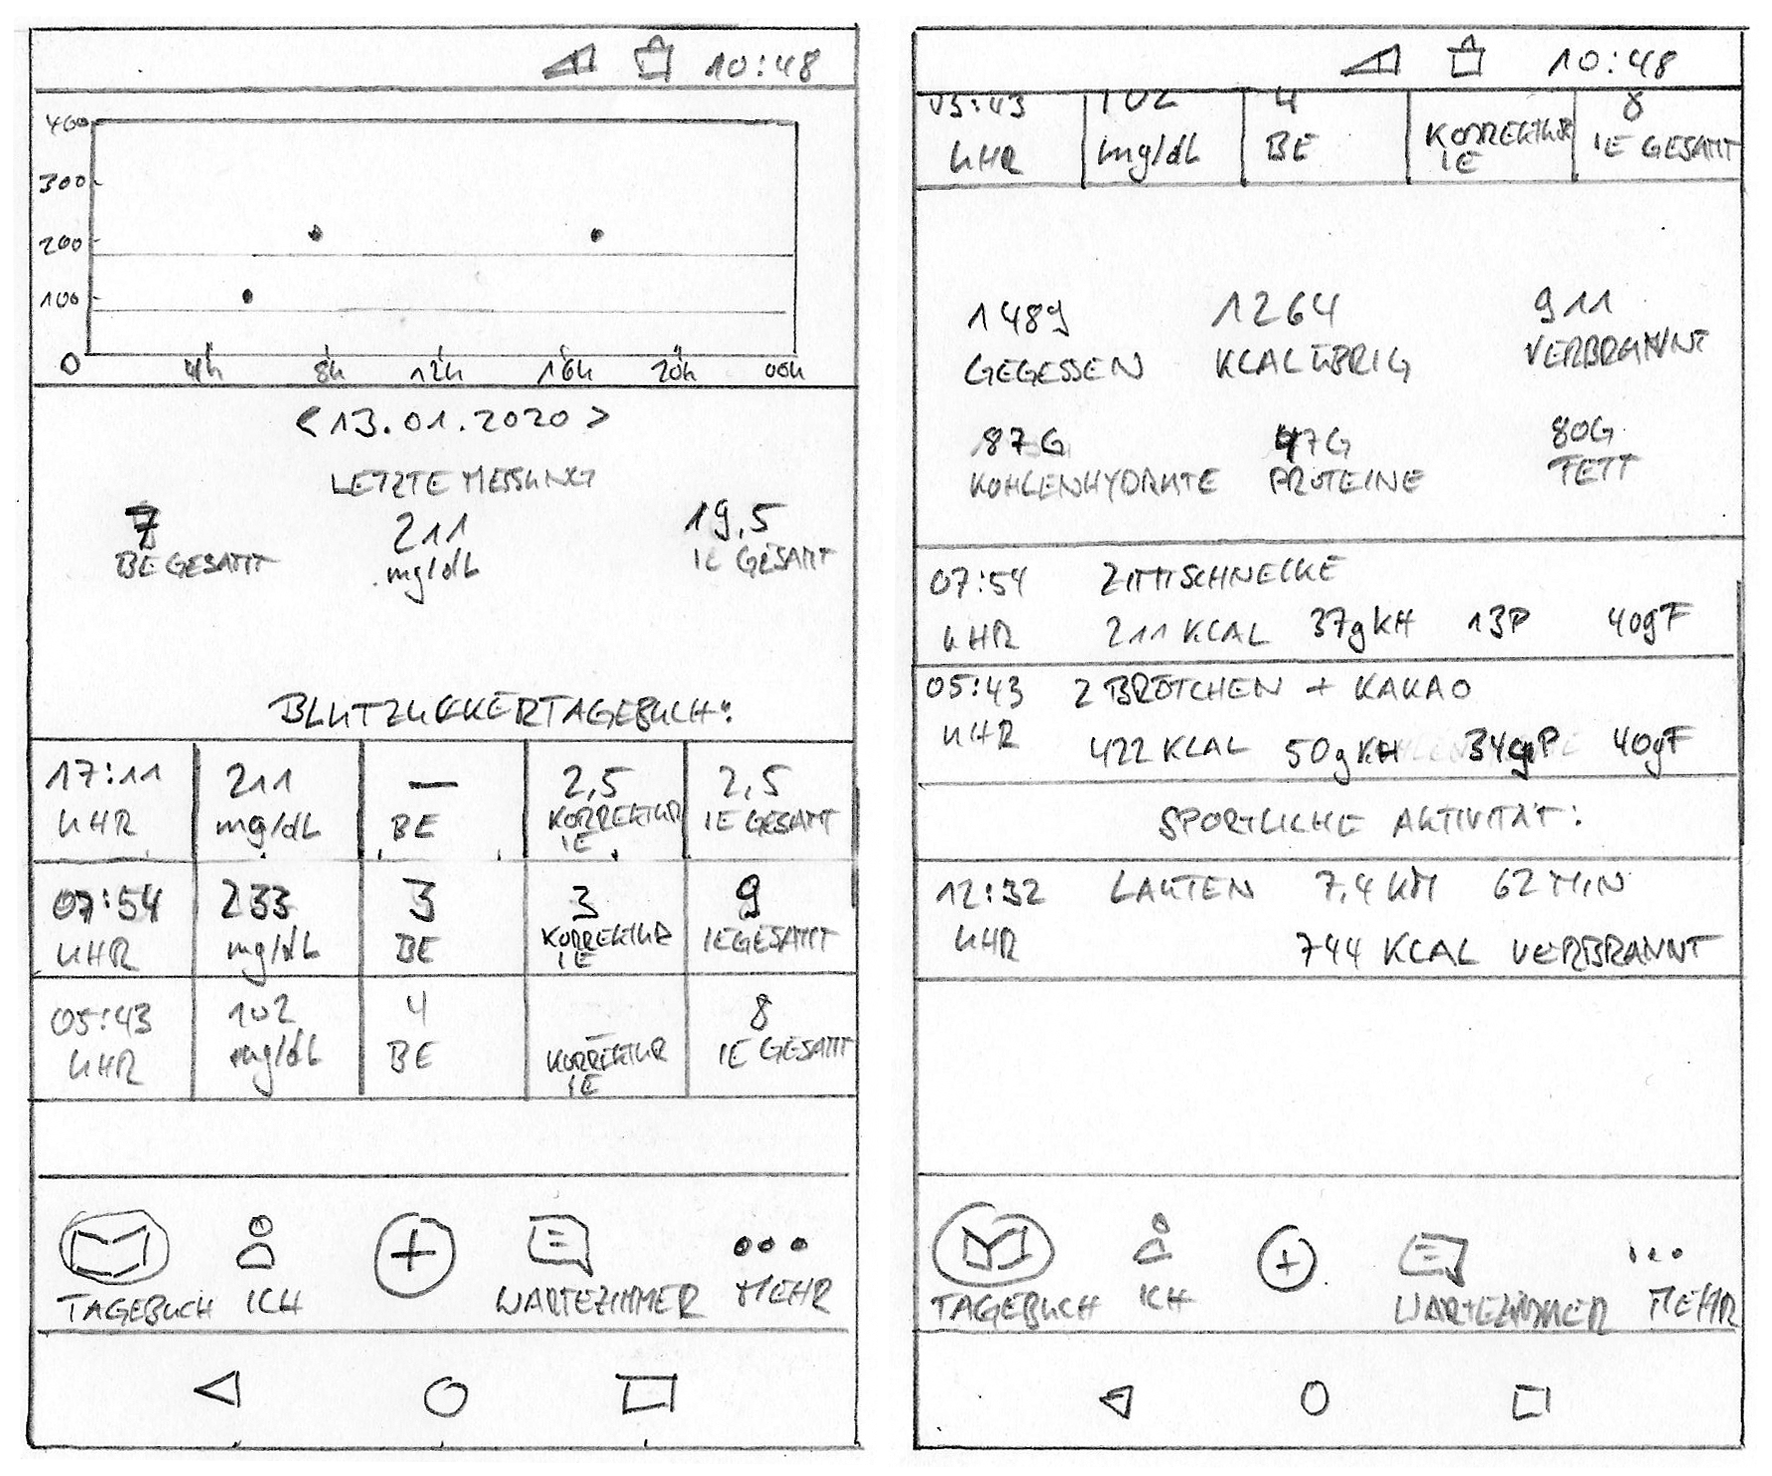
\includegraphics[width=0.6\textwidth]{images/tagebuchscreen.png}
	\captionsetup{justification=centering}
	\caption{Tagebuch-Screen}
	\label{img:tagebuchscreen}
\end{figure}
\begin{figure}[H]
	\centering
	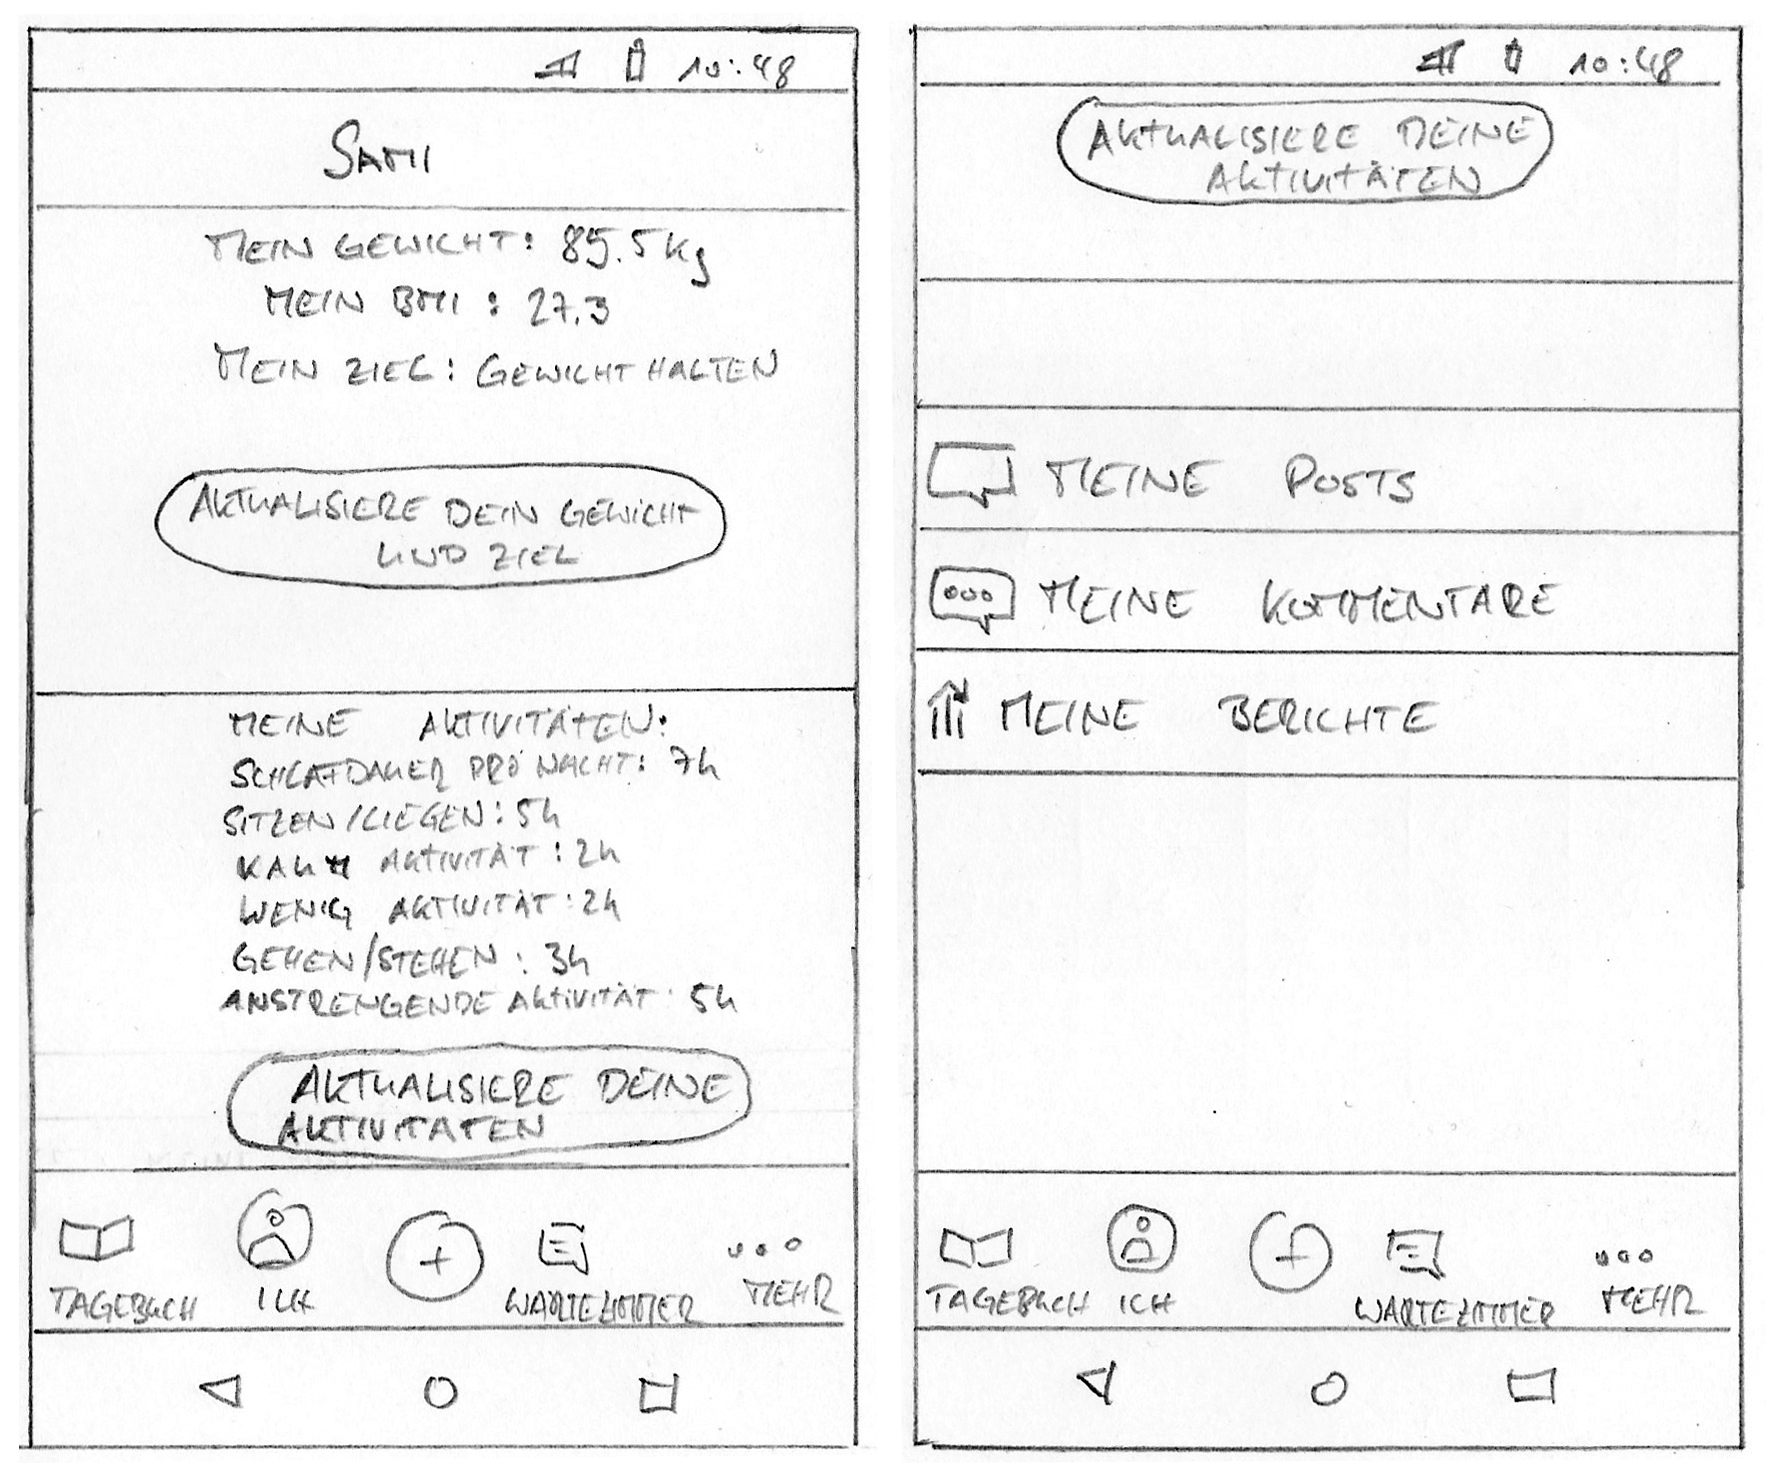
\includegraphics[width=0.6\textwidth]{images/ichscreen.png}
	\captionsetup{justification=centering}
	\caption{Ich-Screen}
	\label{img:ichscreen}
\end{figure}
\begin{figure}[H]
	\centering
	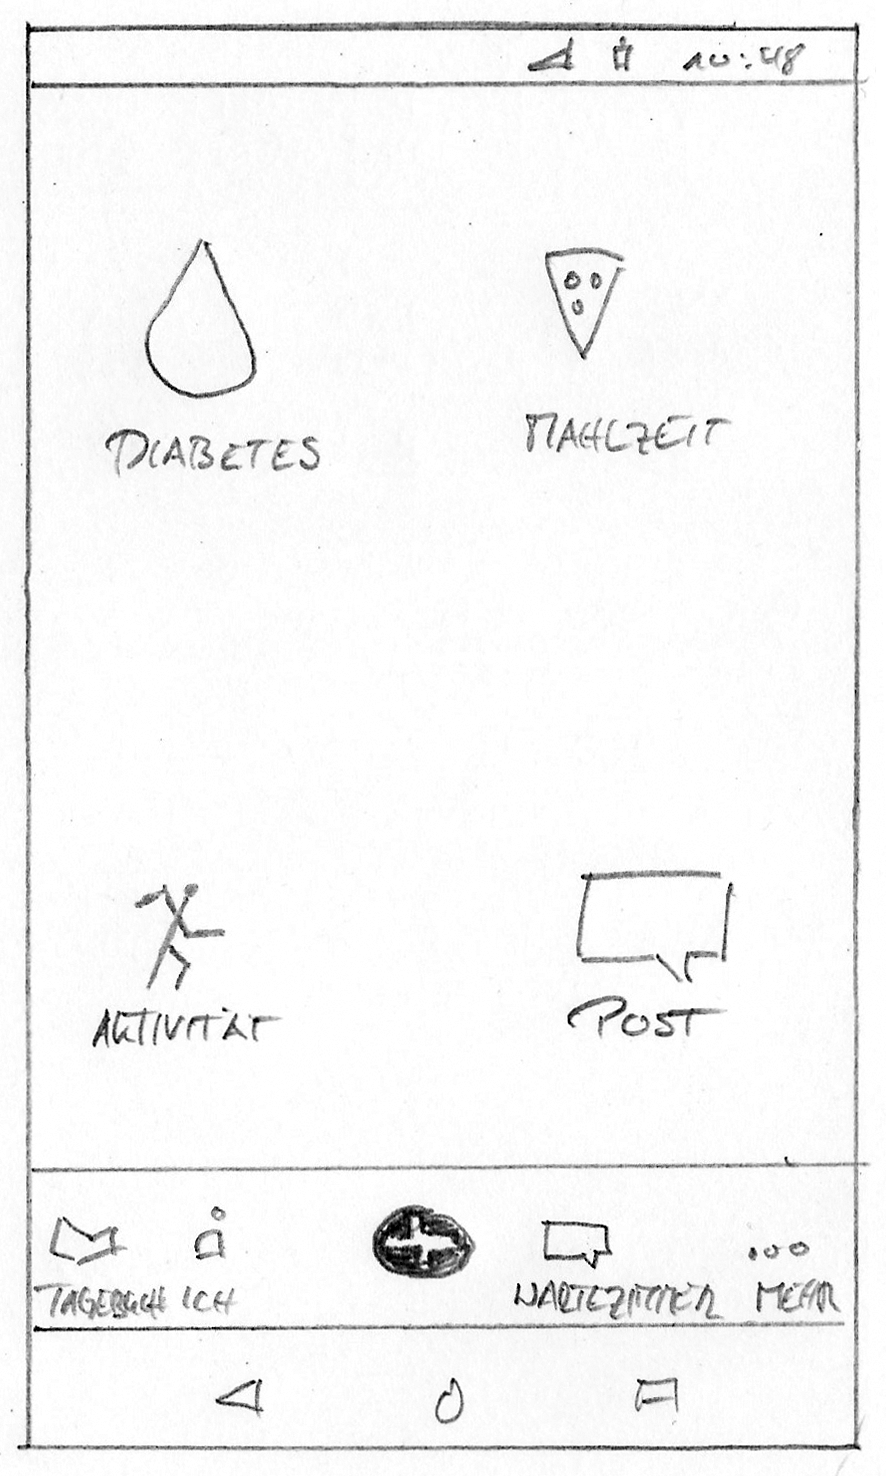
\includegraphics[width=0.3\textwidth]{images/addscreen.png}
	\captionsetup{justification=centering}
	\caption{Add-Screen}
	\label{img:addscreen}
\end{figure}
\begin{figure}[H]
	\centering
	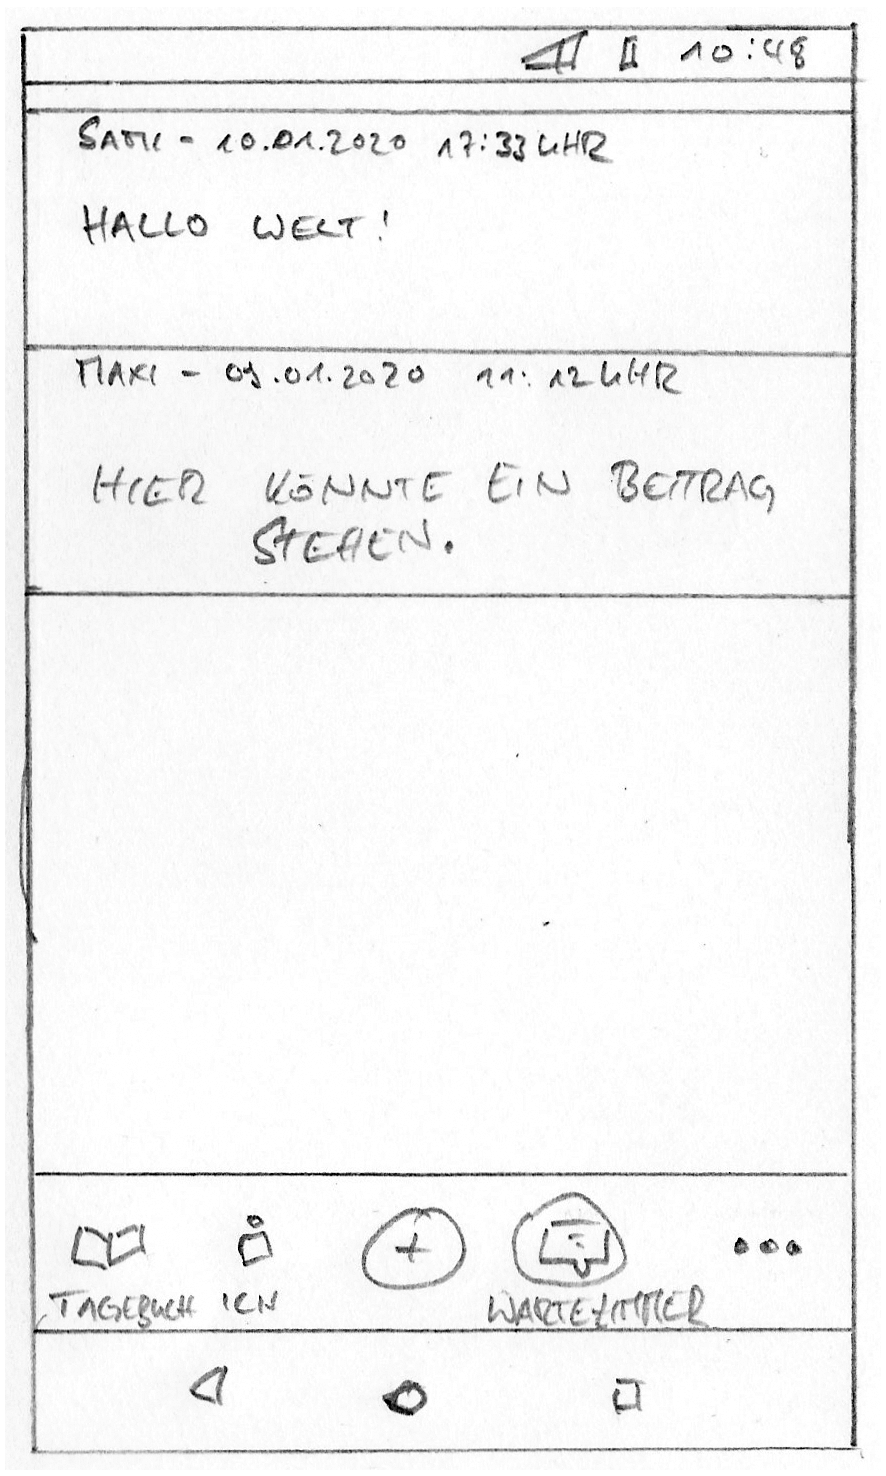
\includegraphics[width=0.3\textwidth]{images/wartezimmerscreen.png}
	\captionsetup{justification=centering}
	\caption{Wartezimmer-Screen}
	\label{img:wartezimmerscreen}
\end{figure}
\begin{figure}[H]
	\centering
	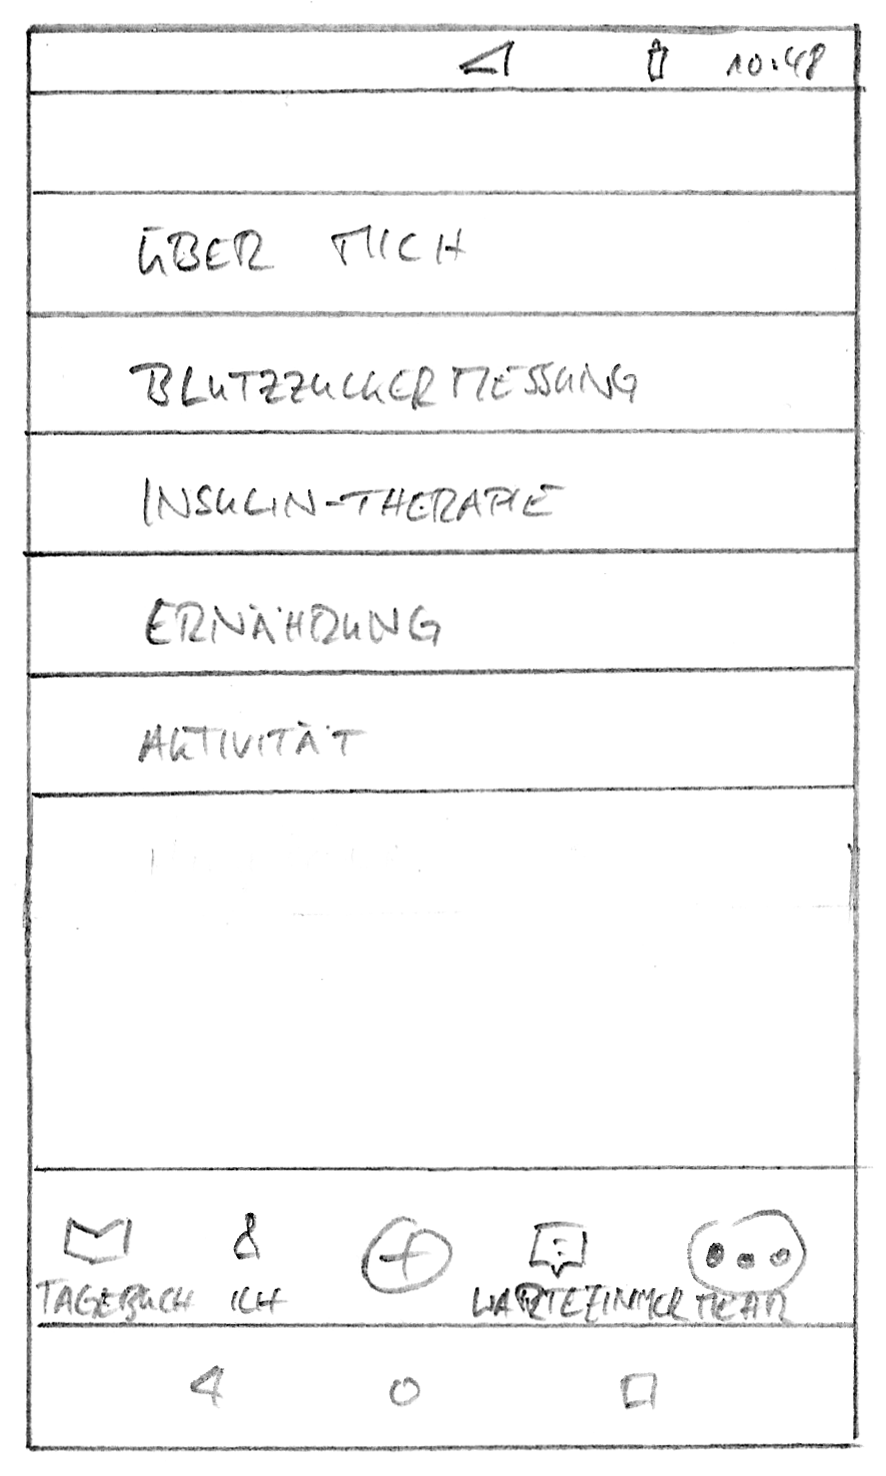
\includegraphics[width=0.3\textwidth]{images/mehrscreen.png}
	\captionsetup{justification=centering}
	\caption{Mehr-Screen}
	\label{img:mehrscreen}
\end{figure}
Die Begriffswahl für „Tagebuch“ (Abbildung \ref{img:tagebuchscreen}: \nameref{img:tagebuchscreen}) ensteht aus der Domäne, das Diabetiker „Tagebucheinträge“ verfassen.  „Ich“ (Abbildung \ref{img:ichscreen}: \nameref{img:ichscreen}) repräsentiert benutzerbezogene Daten und „Wartezimmer“ (Abbildung \ref{img:wartezimmerscreen}: \nameref{img:wartezimmerscreen}) ist eine metaphorische Bezeichnung für eine Treffpunkt verschiedener Benutzer. Unter „Mehr“ (Abbildung \ref{img:mehrscreen}: \nameref{img:mehrscreen}) sind wiederum benutzerbezogene Einstellungen zu bearbeiten. Durch die verschiedenen Navigationspfade soll der Benutzer durch stets angemessene Informationen innerhaln angemessener Zeit auf dem Laufenden gehalten werden.\\
Nach dem Conceputal Model Design folgt das Conceptual Model Mock-Up und die Iterative Conceptual Model Evaluation, in denen die ersten Entwürfe eines Designs mit Stift und Papier erstellt  und anhand von Probanden evaluiert werden. Da allerdings gibt der begrenzte Zeitrahmen diese zwei Arbeitschritte nicht her, wodurch die Abbildungen als Mock-Up dienen und eine Evaluation nicht durchgeführt werden kann. Folglich werden Screen Design Standards festgelegt und anhand dessen ein Style Guide erstellt.
\subsection{Screen Design Standards (SDS)}
Mithilfe der aus der Benutzer- und Aufgabenmodellierung stammenden Erkenntisse und dem Conceptual Model Design werden systemspezifische Standards und Konventionen für alle Aspekte des detaillierten Screen-Designs entwickelt. Dazu dienen die Screen Design Standards als Grundlage der Usability auf dem gesamten User Interface. Das zu entwickelnde System soll folgende Control und Dialog Box Standars aufweisen:\\
\centerline{\textbf{Control Standards}}
\begin{center}
	\begin{longtable}[H]{p{8cm}p{6cm}}
		\textbf{Menu Contents} & \textbf{Control}\\
		\toprule
		Navigationsaktionen & Icon buttons\\
		Eingabe von Zahlen & EditText mit möglicher Eingabe von Zahlen/Seekbar\\
		Eingabe von Dezimalzahlen &  EditText mit möglicher Eingabe von Dezimalzahlen/Seekbar\\
		Eingabe von Text & EditText mit Auswahl von Buchstaben\\
		Auswahl eines Datums & DatePickerDialog\\
		Auswahl einer Uhrzeit & TimePickerDialog\\
		Liste mit Variablent & Spinner/RecyclerView und CardView\\
		\bottomrule
		\captionsetup{justification=centering}
		\caption{Control Standards}
		\label{tab:controlstandars}
	\end{longtable}
\end{center}
\centerline{\textbf{Dialog Box Standards}}
\begin{itemize}
	\item Alle Dialogfelder haben einen blauen Hintergrund.
	\item Titel der Menüleisten, die aufgerufen wurden, werden linksbündig in der Titelleiste geordnet.
	\item Vertikale Gruppen logisch zusammengehöriger Felder.
	\item Zentrierte Ausrichtung von Beschriftungen in Feldgruppen und Feldern, wobei Leeraum zwischen Beschriftungen und Feldern zu minimieren und Größbuchstaben für alle Hauptwörter in Beschriftungen zu verwenden sind.
\end{itemize}
Unter berücksichtigung dieser Standards könnten Dialog Boxes aussehen wie in Abbildung \ref{img:dialogbox}: \nameref{img:dialogbox}.
\begin{figure}[H]
	\centering
	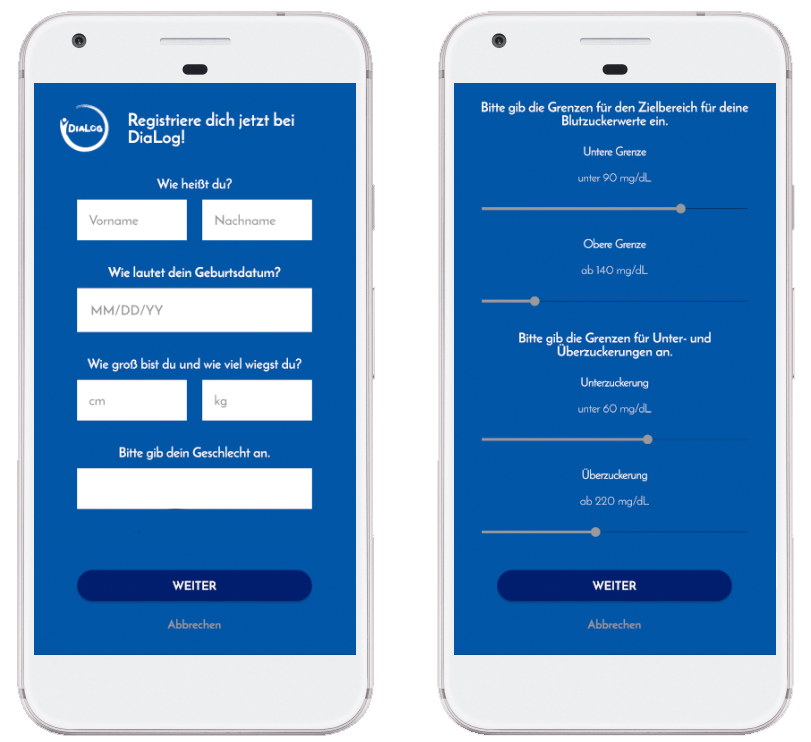
\includegraphics[width=0.5\textwidth]{images/DialogBox.png}
	\captionsetup{justification=centering}
	\caption{Dialog Boxes}
	\label{img:dialogbox}
\end{figure}
Hinzu kommen folgende Standards:
\begin{itemize}
	\item Verwendung von Gruppenfelder und Einbettung von Titeln mit Großbuchstaben in der oberen Mitte des Gruppenfeldes.
	\item Gruppierte boxes von links nach rechts und von oben nach unten entsprechend der natürlichen Reihenfolge oder der erwarteten Verwendungshäufigkeit geordnet.
	\item Weiter push button immer in der unteren Mitte und über dem Abbrechen push button plaziert, wobei alle push buttons gleichmäßig von einander entfernt sind.
	\item Hintergrundfarbe für Eingabefelder:\newline
		\noindent\hspace*{10mm}Read-only - blau \newline
		\noindent\hspace*{10mm}Erforderlich - weiß \newline
		\noindent\hspace*{10mm}Optional - grau 
\end{itemize}

\subsection{Style Guide}
Um nun die Screen Design Standards zu vervollständigen, wird ein Style Guide erstellt. Dieser fügt dem User Interface folgende Kriterien hinzu:\\

\begin{itemize}
	\item Das zu entwickelnde System wird für die Plattform Android entwickelt und soll für alle Betriebssyteme höher als Android 7.0 Nougat kompatibel sein.
	\item Die Displaygröße des Endgerätes muss mindestens 5 Zoll groß sein.
	\item Als primäre Farbe dient blau, aus sekundäre hellblau. Um Akzente zu setzen wird ein Grauton verwendet. Text und Eingabefelde sind gundsätzlich weiß.
	\item Als Eingabe Gerät dient die virtuelle Tastatur in Form des Touchscreens des Endgerätes.
	\item Jeglicher Text wird mit der Font-Familiy Josefin Sans dargestellt. Verschiedene Textarten besitzen folgende Kriterien:\newline
	\noindent\hspace*{10mm}1. Überschrift: 22dp und Bold\newline 
	\noindent\hspace*{10mm}2. Überschrift: 17dp und Semibold\newline 
	\noindent\hspace*{10mm}Text: 15dp und Light\newline
	\noindent\hspace*{10mm}Hinttext von EditText: 17dp und Semibold\newline
	\noindent\hspace*{10mm}Buttons: 15dp und Bold\newline   
	\noindent\hspace*{10mm}Klickbare Texte: 15dp und Bold 
	\item Buttons und Menüpunkte sollen mit Objekten, wie ein Buch-Icon für das Tagebuch, versehen werden, um den kognitiven Arbeitsaufwand des Benutzers zu reduzieren.
	\item Interaktionen vom Benutzer mit dem System soll sich das System merken können, sodass bei der Suche nach einem Lebensmittel die letzten verwendeten Lebensmittel vorgeschlagen werden.
	\item Dem Benutzer sollte wenn möglich Eingaben vorgegeben werden. So sollen beispielsweise BE/KE oder Insulineinheiten vorberechnet werden und bei der Eingabe von Uhrzeiten und Daten die aktuellen Parameter vorgeschlagen werden. Dabei soll der Benutzer diese jedoch noch anpassen können.
	\item Der Benutzer sollte sich keine Informationen von einem Teil eines Dialogs zum nächsten merken müssen.
	\item Der Benutzer sollte immer zu dem vorherigen Layout zurückkehren können.
\end{itemize}
Mithilf der festgelegten Screen Design Standards und den definierten Style Guide ist nun das Detailed User Inteface Desing zu gestalten.
\subsection{Detailed User Interface Design (DUID)}
	Das Detailed User Interface Design ist das endgültige Design der Benutzeroberfläche. Die bisherigen Ergebnisse aus der Benutzer- und Aufgabenmodellierung, dem Conceptual Model Design, den Screen Design Standards und dem Style-Guide fließen alle in das detaillierte Design der Benutzeroberfläche (Detailed User Interface Design) ein.\newline
	Das System wird wie folgt mit fünf verschiedenen main screens implementiert:
\begin{itemize}
	\item Tagebuch-Screen (Abbildung \ref{img:DUIDtagebuchscreen}: \nameref{img:DUIDtagebuchscreen})
	\item Ich-Screen (Abbildung \ref{img:DUIDichscreen}: \nameref{img:DUIDichscreen})
	\item Add-Screen (Abbildung \ref{img:DUIdreiscreen}: \nameref{img:DUIdreiscreen})
	\item Wartezimmer-Screen (Abbildung \ref{img:DUIdreiscreen}: \nameref{img:DUIdreiscreen})
	\item Mehr-Screen (Abbildung \ref{img:DUIdreiscreen}: \nameref{img:DUIdreiscreen})
\end{itemize}
Die folgenden Änderungen wurden am Konzeptmodelldesign (CM Design) vorgenommen:
\begin{itemize}
	\item Jeder Screen hat einen Titel, sodass der Benutzer jederzeit sehen kann, auf welchem Bildschirm er sich befindet.
	\item Auf jedem Screen in der oberen rechten Ecke wird dem Benutzer seine Punktzahl angezeigt. Er dient dem Wettbewerb zwischen Nutzern und kann durch Interaktion mit dem System gesteigert werden. Auf diese Weise erhält der Benutzer beim Schreiben von Beiträgen oder Ereignissen immer Belohnungspunkte. Dies soll den Benutzer ermutigen, das System zu verwenden.
\end{itemize}
	Der Tagebuch-Screen (Abbildung \ref{img:DUIDtagebuchscreen}: \nameref{img:DUIDtagebuchscreen}) zeigt die tägliche Dokumentation von Blutzuckerwerten, Mahlzeiten und sportlichen Aktivitäten. Diese ist eine Bildlaufansicht (ScrollView), um alle erforderlichen Informationen in einem Layout darstellen zu können. Durch Ändern des Datums kann der Benutzer jederzeit die Daten eines anderen Tages anzeigen und bearbeiten. Die Blutzuckerwerte werden in Form eines Koordinatensystems und einer Tabelle dargestellt. Das Koordinatensystem zeigt alle Blutzuckerwerte für den ausgewählten Tag an und in der Tabelle wird jeder Datensatz um die Uhrzeit, die aufgenommenen BE's/KE's und die injizierten Korrektur- und Gesamtinsulineinheiten ergänzt. Die tabellarische Darstellung ergibt sich aus einer Recycler-Ansicht (RecyclerView), die die Liste der Blutzuckerwerte in Form einer Kartenansicht (CardView) enthält.\newline
	Neben den Mahlzeiten werden dem Benutzer auch seine offenen, verbrannten und aufgenommenen Kalorien angezeigt. Die Views für sportliche Aktivitäten werden um die Uhrzeit und den Kalorienverbrauch ergänzt.\newline
	Ebenso wie die Blutzuckerwerte und die sportlichen Aktivitäten werden Mahlzeiten in Recycler- und CardReviews präsentiert, die die Uhrzeit, die Beschreibung von Lebensmitteln und deren Kalorien, Kohlenhydrate, Proteine und Eiweiße beinhalten. Alle drei Informationskategorien werden gruppiert dargestellt.

\begin{figure}[H]
	\centering
	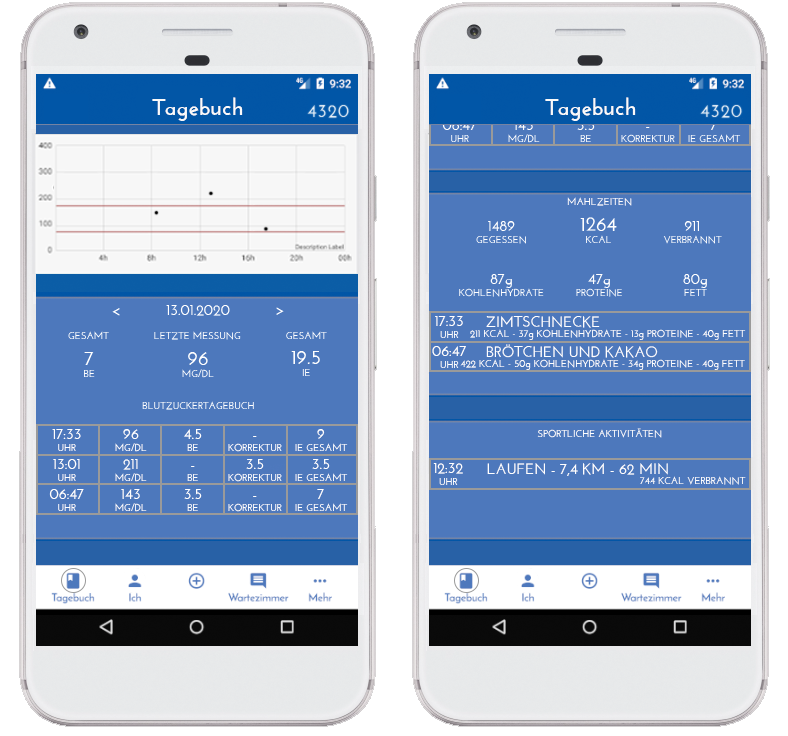
\includegraphics[width=0.5\textwidth]{images/tagebuchscreen_digital.png}
	\captionsetup{justification=centering}
	\caption{DUID: Tagebuch-Screen}
	\label{img:DUIDtagebuchscreen}
\end{figure}
In den restlichen Screens sind kaum Veränderungen zum Conceptual Model Design entstanden. Farben und Title wurden hinzugefügt, Information wurden gruppiert und voneinander abgegrenzt und Symbole und Icons wurden ausgetauscht. Im Folgenden sind die einzelnen Detailed User Inferface Designs zusehen:\\
\begin{figure}[H]
	\centering
	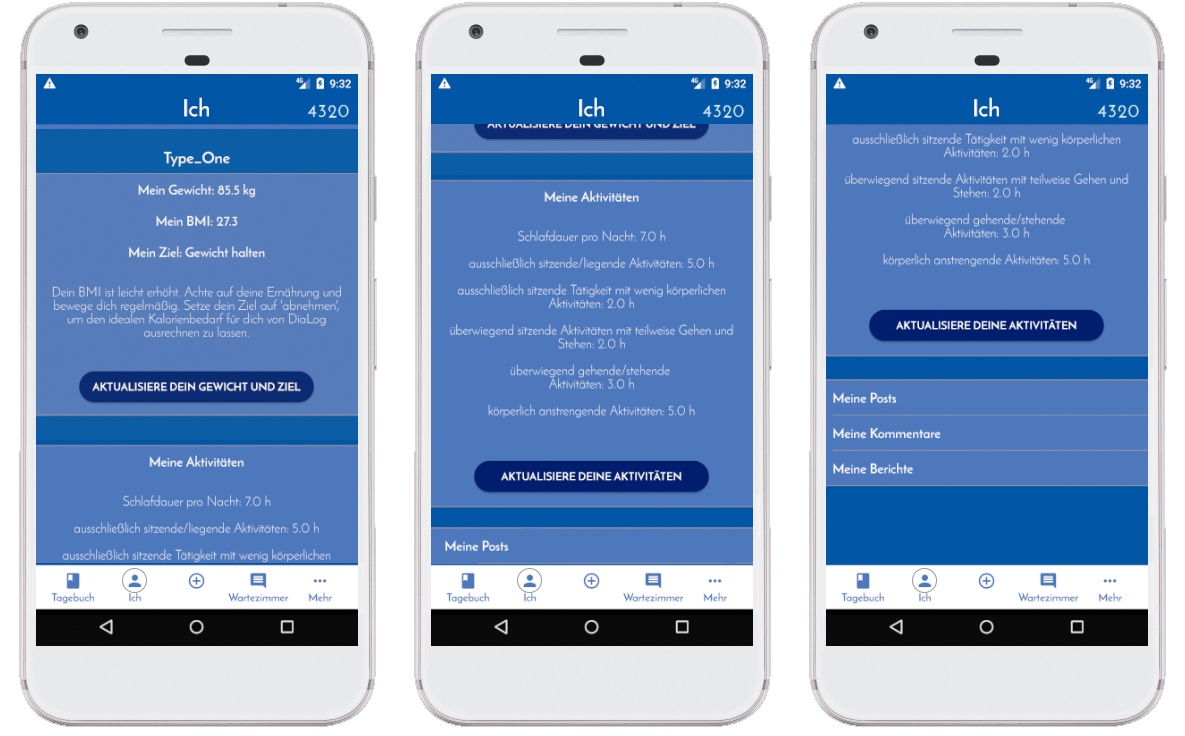
\includegraphics[width=0.75\textwidth]{images/ichscreen_digital.png}
	\captionsetup{justification=centering}
	\caption{DUID: Ich-Screen}
	\label{img:DUIDichscreen}
\end{figure}
\begin{figure}[H]
	\centering
	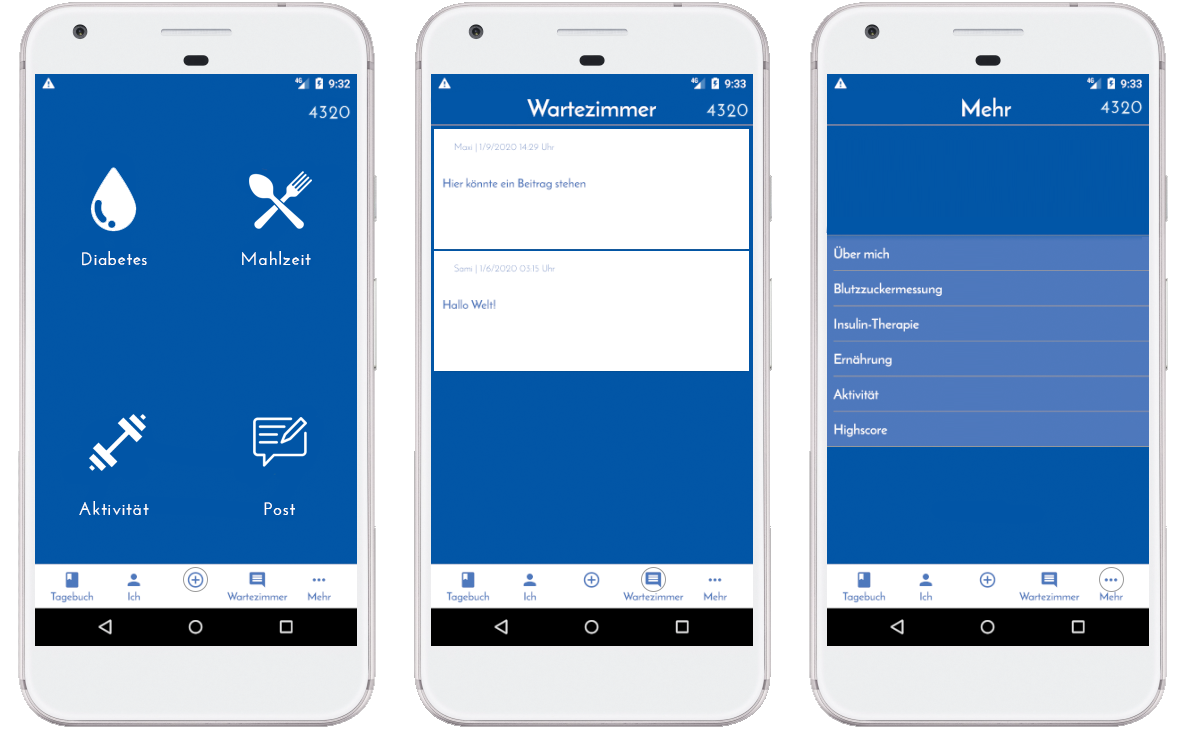
\includegraphics[width=0.75\textwidth]{images/drei_digital.png}
	\captionsetup{justification=centering}
	\caption{DUID: Add-, Wartezimmer- und Mehr-Screen (von links nach rechts)}
	\label{img:DUIdreiscreen}
\end{figure}



